\chapter{Processi stocastici}
I processi stocastici costituiscono una classe di modelli di sistemi che permette lo
studio e l’analisi dei sistemi. In questo Capitolo verranno riportate alcune definizioni e classificazioni dei suddetti processi, soffermando l'attenzione sui processi Markoviani.

\section{Processi stocastici}
Un \textbf{processo stocastico} è definito come una famiglia di variabili casuali $X = \{X(t) | t \in T\}$ definite in uno \textbf{spazio di probabilità} $\Omega$ ed indicate dal parametro \textbf{t}, dove t varia in un insieme T e indica il tempo. Ogni variabile casuale X(t) assume valori, detti \textbf{stati}, in un insieme E detto \textbf{spazio degli stati} del processo stocastico. Essendo che ogni variabile è definita come una funzione su uno spazio campione S, allora il processo stocastico è visto come un insieme di funzioni $\{ X(t,s) | t\in T, s \in S\}$.\\
I processi stocastici possono essere classificati in base alle seguenti caratteristiche:
\begin{itemize}
    \item spazio degli stati E
    \item indice tempo
    \item tipo di dipendenza stocastica fra le variabili casuali
\end{itemize}

\subsection{Spazio degli stati E}
Lo spazio degli stati può essere \textbf{discreto} o \textbf{continuo}. Nel primo caso il processo è detto anche catena e lo spazio E è indicato come l'insieme di interi non negativi. Nel secondo l'insieme dei valori assunti non è finito o numerabile perciò il processo è a spazio continuo.
\subsection{Indice tempo}
L'indice tempo è a sua volta \textbf{discreto} o \textbf{continuo}. Un processo a tempo discreto è anche detto sequenza stocastica ed è denotato come $\{X_n | n \in T \}$ dove T è finito o numerabile. Al contrario, se i cambiamenti avvengono in un qualsiasi istante di un tempo infinito allora si ha un processo a tempo continuo e si denota come $\{ X(t) | t\in T\}$.

\subsection{Dipendenza stocastica fra variabili}
La \textbf{dipendenza stocastica} fra variabili casuali X(t) per diversi valori di t è identificata dalla funzione di distribuzione di probabilità congiunta per le variabili $X= [X(t_1),X(t_2),...,X(t_n)]$, vedi \ref{subsec:prob_congiunta}, denotata come:
\[F_X(x;t) = Prob\{ X(t_1) \leq x_1; X(t_2) \leq x_2; ... ; X(t_n) \leq x_n \}\]
al variare di n e di $x= [x_1,x_2,...,x_n]$ e  $t= [t_1,t_2,...,t_n]$ con $x_i \in E$, $t_i \in T$ $1 \leq i \leq n$, $ n \geq 1$ e $t_1 \leq t_2 \leq ... \leq t_n$.

\subsubsection{Classificazione in base alla dipendenza stocastica}
Come accennato in precedenza è possibile classificare i processi in base alla dipendenza stocastica. \\
Un processo si dice \textbf{stazionario} in senso stretto se la funzione distribuzione $F_X (x;t)$ è invariante rispetto allo spostamento sull'asse del tempo T ovvero se per ogni $\tau$ costante
\[F_X (x; t+\tau) = F_X(x;t)\]
dove $t + \tau = [t_1+ \tau,t_2+\tau,...,t_n+\tau]$ e per ogni x,t e n.\\
Un processo stocastico è \textbf{indipendente}  se la funzione di distribuzione congiunta è
fattorizzabile nelle singole funzioni di distribuzione marginali:
\[ F_X(x;t)= \prod_{i=1}^{n} F_{X_{i}}(x_i;t_i) = \prod_{i=1}^{n} Prob\{ X(t_i) \leq x_i\}\]
Un processo stocastico è di\textbf{ rinnovamento} se le variabili casuali $X_1,X_2,...$ sono indipendenti, identicamente distribuite e a valori non negativi.

\subsection{Processi di Markov}
Un processo stocastico a tempo discreto $\{X_n |n \in T \}$ è di Markov se la probabilità di stato al tempo n+1 dipende soltanto dallo stato al tempo attuale,n, e non dalla storia precedente, ovvero se per ogni $n >0$ e per ogni valore degli stati $j,i_0,i_1,i_2,..., i_n \in E$ si ha:
\[Prob\{X_{n+1} = j | X_0 = i_0; X_1=i_1;...;X_n = i_n\} = Prob \{ X_{n+1} = j |X_n =i_n\}\]

Un processo stocastico a tempo continuo $\{X_n |n \in T \}$ è di Markov se per ogni sequenza di valori $t_0 \leq t_1\leq... \leq t_n< t$ la distribuzione di probabilità di X(t) condizionata a $X(t_0),X(t_1),..., X(t_n)$ dipende soltanto dallo stato $X(t_n)$, per ogni $n >0$ e per ogni valore degli stati $j,i_0,i_1,i_2,..., i_n \in E$ si ha:
\[Prob\{X(t) = j | X(t) = i_0; X(t_1)=i_1;...;X(t_n) = i_n\} = Prob \{ X(t) = j |X(t_n) =i_n\}\]

Per un processo di Markov a tempo discreto il tempo di permanenza in uno stato è un v.c. \textbf{geometrica} mentre per un processo di Markov a tempo continuo è un v.c. \textbf{esponenziale}. Questo vincolo deriva
dalla proprietà di assenza di memoria indotta sulla v.c. dal processo Markoviano. Come è noto le uniche distribuzioni che godono della proprietà di assenza di memoria sono, rispettivamente, la geometrica fra le distribuzioni discrete e l’esponenziale fra le continue. Se si assume che la distribuzione di probabilità non sia geometrica o esponenziale allora si ha un processo stocastico di semi-Markov, in questo caso le transizioni di tempo vanno ad istanti di tempo presi arbitrariamente. \\
Un p.s. di Markov a spazio discreto E è anche detta \textbf{catena di Markov}.
Una catena di Markov è di \textbf{nascita-morte} (birth-death) se le uniche transizioni possibili che il processo può effettuare sono soltanto fra stati vicini. Nel caso di tempo discreto, se lo stato $X_n=i$ allora lo stato al tempo successivo può soltanto essere $X_{n+1}\in{i-1, i, i+1}$. \\
Se lo spazio degli stati E è a tempo discreto allora $\{X_n | n \in N\}$ è una catena di Markov a tempo discreto, $X_n = j$ indica che il processo si trova nello stato j al tempo n, $n \in N$, $j \in E$. Nella formula della probabilità condizionata al membro destro:
\[Prob\{X_{n+1} = j | X_n = i\}\]

è detta probabilità di transizione al tempo n dallo stato i allo stato $j,i,j\in E, n \geq 0$.
Una catena di Markov si dice omogenea se le probabilità di transizione sono indipendenti dal tempo n. La probabilità di transizione dallo stato i allo stato j è definita come:
\[ p_{ij} = Prob\{X_{n+1} = j | X_n = i\}\]
$\forall i,j \in E, \forall n \geq 0$. \\
Una catena di Markov può essere analizzata sia in un tempo finito (\textbf{analisi transiente}, non importante per esame) sia a lungo termine (\textbf{analisi stazionaria}).

\subsection{Analisi stazionaria}
La descrizione del processo stocastico in condizioni asintotiche, per il tempo n che tende ad infinito, si esprime in termini di distribuzione di probabilità di stato. Sia $ \pi_j = \lim_{n \to \infty} \pi_j(n) = Prob\{X=j\}$ la probabilità di osservare lo stato j in condizioni di equilibrio, $\forall j \in E$. In forma compatta indichiamo con $\pi =[\pi_0, \pi_1. \pi_2,...,\pi_n]$ il vettore delle probabilità stazionarie di stato.

\subsubsection{Classificazione degli stati}
\begin{figure}[H]
	\centering
    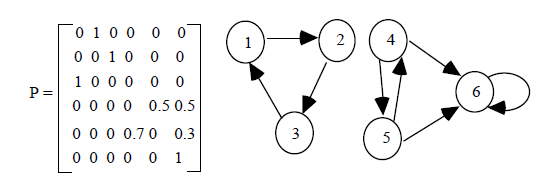
\includegraphics[width=15cm, keepaspectratio]{img/diagramma_Markov.png}
	\caption{Esempio di diagramma fra gli stati di una catena di Markov a tempo discreto
con matrice delle probabilità di transizione P.}\label{fig:diagr_Markov}
\end{figure}

In Fig.\ref{fig:diagr_Markov} il sottoinsieme E'={1,2,3} è chiuso, gli stati 1, 2 e 3 sono ricorrenti periodici di periodo 3. Gli stati 4 e 5 sono transienti e lo stato 6 è assorbente.

\paragraph{Teorema}
La distribuzione di probabilità stazionaria $pi$ di una catena di Markov omogenea, irriducibile e aperiodica \footnote{Uno stato ricorrente è\textbf{ aperiodico} se $g_i=1$ ed è periodico se $g_i>1$.} esiste sempre ed è indipendente dallo stato iniziale. Inoltre
\begin{itemize}
    \item se gli stati sono transienti \footnote{Uno stato i è \textbf{transiente} se vi è probabilità non nulla di non ritorno allo stato i.} o ricorrenti \footnote{Uno stato $i\in E$ è \textbf{ricorrente} se il processo, iniziando nello stato i, torna allo stato i con certezza (con probabilità 1).} nulli allora $\pi_j = 0$, $\forall j \in E$, e non esiste distribuzione stazionaria;
    \item se gli stati sono ricorrenti non-nulli allora $\pi_j > 0$, $\forall j \in E$, e la distribuzione stazionaria $\pi$ è l'unica soluzione non negativa del sistema lineare
    \[ \pi = \pi P\]
    con la condizione di normalizzazione $\sum j\pi_j = 1$.
\end{itemize}


\paragraph{Teorema}
Per una catena di Markov a tempo continuo omogenea, irriducibile ed aperiodica esiste sempre la probabilità stazionaria di stato $\pi_j = \lim_{t \to \infty} \pi_j (t), j\in E$, ed è indipendente dallo stato iniziale.
La soluzione stazionaria si ottiene allora imponendo $\frac{\mathrm{d \pi(t)} }{\mathrm{d} t} = 0$ da cui, dalla
equazione $\frac{\mathrm{d \pi (t)} }{\mathrm{d} t} = \pi(t) Q$ deriva
\[\pi Q = 0\] \label{eq:eq_bilanciamento_globale}
che, insieme alla condizione di normalizzazione $\sum i \pi_i = 1$, determina univocamente la soluzione.


Il sistema di equazioni \ref{eq:eq_bilanciamento_globale} è detto anche sistema di \textbf{equazioni di bilanciamento globale} in quanto la singola equazione relativa allo stato i può essere riscritta come:
\[\pi_i \sum_{j\neq i}^{} q_{ij} = \sum_{j \neq i}^{} \pi_j q_{ij}\]
Questo vuol dire che la probabilità di entrare in un stato i è uguale alla probabilità di uscire da quest'ultimo.
Tale equazione si può interpretare come bilanciamento fra il flusso totale uscente dallo stato i (membro sinistro) e il flusso totale entrante in i e proveniente da tutti gli altri stati $j\neq i$ (membro destro).\\
Al contrario il bilanciamento locale è soddisfatto da una catena di Markov se sono uguali il flusso di probabilità da uno stato i a uno stato j e viceversa, ovvero se per ogni $i,j \in E$:
\[\pi_i q_{ij}= \pi_{j} q_{ij}\]

\subsubsection{Processi di nascita-morte}
In una catena di Markov di nascita-morte (birthdeath), con spazio degli stati E=N, le uniche transizioni fra stati ammesse sono dallo stato i agli stati i-1, i, i+1, $\forall i \in E$.

\begin{figure}[H]
	\centering
    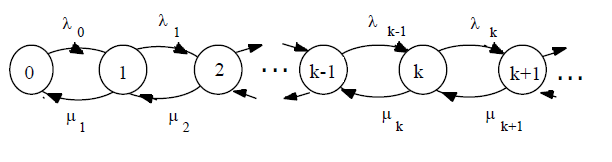
\includegraphics[width=15cm, keepaspectratio]{img/process_nasc_morte.png}
	\caption{Processi di nascita-morte.}\label{fig:nascita_morte}
\end{figure}


Consideriamo un processo di nascita-morte a tempo continuo. In tal caso definiamo la matrice $Q = [q_{ij}]$ delle velocità di transizione fra stati i,$j\in E$, come:
\begin{align}
    & q_{i i+1} = \lambda_i & i \geq 0\\
    &q_{i i+1} = \mu_i & i \geq 0\\
    & q_{00} = -\lambda_0&\\
    & q_{ii} = -(\lambda_i + \mu_i) & i \geq 1\\
    & q_{ij} = 0 & \textrm{per}  |i-j| >1
\end{align}
Il processo è omogeneo perché questi tassi dipendono solo dallo stato e non dal tempo.\\
Il sistema di equazioni $\frac{\mathrm{d \pi (t)} }{\mathrm{d} t} = \pi(t) Q$  relativo alla distribuzione di probabilità di stato $\pi(t)$ al tempo t>0 per un processo di nascita e morte assume la forma seguente:
\begin{align}
    & \frac{\mathrm{d \pi_0 (t)} }{\mathrm{d} t} =  \mu_1 \pi_1(t) -\lambda_0 \pi_0(t) \\
    & \frac{\mathrm{d \pi_k (t)} }{\mathrm{d} t} =  \lambda_{k-1} \pi_{k-1}(t) + \mu_{k+1} \pi_{k+1}(t) - (\lambda_k + \mu_k) \pi_k(t)   & k >0\\
\end{align}

Questo sistema di equazioni descrive il comportamento del processo in funzione del
tempo e può essere risolto assumendo una distribuzione di probabilità di stato iniziale, riguarda la parte dell'analisi transiente.
\\
Se il processo di nascita e morte è irriducibile la probabilità stazionaria di stato $\pi$ si ottiene dalla soluzione del sistema di equazioni di bilanciamento globale che può essere riscritto come:
\begin{align}
    &\mu_1 \pi_1 = \lambda_0 \pi_0\\
    & \lambda_{k-1} \pi_{k-1} + \mu_{k+1} \pi_{k+1} = (\lambda_k + \mu_k)\pi_k & k>0\\
\end{align}
Questo sistema può essere facilmente risolto ad esempio per sostituzione. Infatti dalla
prima equazione si ricava
\[\pi_1 = \pi_0 \dfrac{\lambda_0}{\mu_1}\]
e per sostituzione, dalla seconda equazione
\[\pi_2 = \pi_1 \dfrac{\lambda_1}{\mu_2} = \pi_0 \dfrac{\lambda_1 \lambda_0}{\mu_2 \mu_1}\]
e, per sostituzioni successive, dall’equazione k-sima
\[\pi_k = \pi_{k-1} \dfrac{\lambda_{k-1}}{\mu_{k}} =\pi_0 \prod_{i=0}^{k-1} \dfrac{\lambda_i}{\mu_{i+1}}\]
per k>0.

\paragraph{Condizione di stazionarietà}
Una condizione necessaria e sufficiente perché il processo di nascita e morte sia
ergodico (irriducibile, aperiodico, ricorrente non nullo)  è che esista un $k_0>0$
tale che $\forall k > k_0 $ sia $\lambda_k < \mu_k$ , ovvero $\rho = \dfrac{\lambda}{\mu} < 1 $. Questo vuol dire che se la velocità degli arrivi è maggiore di quella delle partenze allora il sistema è congestionato.

\subsection{Processo di pura nascita}
Considerando il particolare processo di nascita e morte in cui i tassi di morte sono
nulli ($\mu_k=0, k>0$), definiamo un processo di \textbf{pura nascita}. Assumiamo inoltre che il
tasso di nascita sia costante, indipendente dallo stato:$\lambda_k = \lambda, k \geq 0$.

\begin{figure}[H]
	\centering
    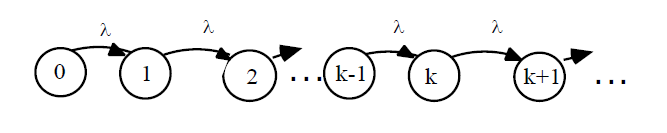
\includegraphics[width=15cm, keepaspectratio]{img/processo_pura_nascita.png}
	\caption{Diagramma di un processo di pura nascita.}\label{fig:diagr_pura_nascita}
\end{figure}

Assumendo la condizione iniziale di sistema vuoto, $\pi_0(0) = 1, \pi_k(0) = 0, \forall k\neq 0$, si ricava facilmente la soluzione transiente:
\begin{align}
    & \pi_k(t)= \dfrac{(\lambda t)^k}{k!} e^{-\lambda t} & k\geq 0, t\geq 0
\end{align}
che riconosciamo, in accordo alla formula \ref{eq:prob_poisson}, come la distribuzione di Poisson di
parametro $\lambda t$, di media e varianza $\lambda tt$.

\subsection{Processo di Poisson}
Indichiamo con N(t), $t\geq0$, il numero di eventi osservati in un intervallo di tempo [0,t], nel caso di un sistema aperto esso rappresenta il numero di arrivi nel suddetto intervallo (\textbf{processo di arrivo}).Inoltre sia $X_i$ la v.c. che indica il tempo che intercorre fra l’arrivo dell’(i-1)-esimo job e l’arrivo dell’i-esimo job al sistema, per i>1, con $X_1$ indichiamo l'arrivo del primo job. Se le v.c. $X_i$, i>0, sono indipendenti ed identicamente distribuite, allora il processo stocastico $\{N(t) | t\geq0\}$ è di rinnovamento. Inoltre se le v.c. $X_i$, i>0, sono i.i.d. con distribuzione esponenziale di parametro $\lambda$ il quale indica il tasso di arrivo, allora il processo stocastico $\{N(t) | t\geq0\}$ è di Poisson. La distribuzione di probabilità di Poisson con parametro $\lambda t$ è data dalla seguente formula:
\[Prob\{N(t) = i\} = e^{-\lambda t} \dfrac{(\lambda t)^i}{i!}\]
\[E[N(t)] = Var[N(t)] = \lambda t\] \label{eq:prob_poisson}
con $i\geq 0$.
Il processo di Poisson può essere definito come il processo stocastico che indica il numero di eventi osservati in un intervallo di tempo [0,t], e che soddisfa le seguenti condizioni:
\begin{itemize}
    \item il numero di eventi in intervalli disgiunti sono stocasticamente indipendenti;
    \item il numero di eventi in un intervallo di tempo dipende solo dalla sua lunghezza e non dall'istante iniziale;
    \item per un valore piccolo di t e per una costante positiva $\lambda$ si ha che:
        \begin{itemize}
             \item Prob \{ un evento in un intervallo di ampiezza t \} = $\lambda t + o(t)$
             \item Prob \{ nessun evento in un intervallo di ampiezza t \} = $o(t)$
             \item Prob \{ più di un evento in un intervallo di ampiezza t \} = $o(t)$ dove $o(t) = \lim_{t \to \infty} [o(t)/t] = 0$.
        \end{itemize}
\end{itemize}
Dalla seconda proprietà deriva che
\[Prob\{ \textrm{k eventi nell'intervallo (s,s+t)}\}= e^{-\lambda t} \dfrac{(\lambda t)^k}{k!}\]
In questo caso se il tempo di interarrivo è esponenziale allora il processo di arrivo è di Poisson e viceversa. Indichiamo con la X la variabile casuale tempo di interarrivo con distribuzione cumulativa $A(t) = Prob\{X \leq t\}$ allora possiamo scrivere che 
\[A(t) = Prob\{N(t) = 0\} = 1 - e^{-\lambda t}, \textrm{ con t>0}\]


\subsubsection{Composizione di processi di Poisson}
La sovrapposizione o composizione di n processi di Poisson indipendenti rispettivamente di parametro $ \lambda_{1}, \lambda_{2} , ..., \lambda_{n}$ è anch’esso un processo di Poisson di parametro $\lambda_{1}+\lambda_{2} +…+\lambda_{n} $.

\subsubsection{Decomposizione di processi di Poisson}
Dato un processo di Poisson $\{N(t) | t\geq 0\}$ di parametro $\lambda$, assumiamo che sia decomposto in n processi, selezionando ogni uscita del processo secondo una distribuzione di probabilità di Bernoulli ad n uscite, con probabilità $p_i, 1\leq i \leq n$. Allora gli n processi di uscita $\{N_i(t)| t\geq 0\} $ sono indipendenti e sono anch'essi processi di Poisson rispettivamente con parametro $\lambda p_i, 1\leq i \leq n$.


